\chapter{Experimental Setup}
\label{experimentalsetup}
%\pagenumbering{arabic} 
The performance of our method is evaluated on the PKU-MMD~\cite{liu2017pku}, a multi-view dataset. The dataset consists of 51 different classes and each action is captured from three different angles. In our experiment, we used only five action classes and multi-view videos. In PKU-MMD dataset each video contains different number of actions that requires video segmentation to segment them into individual action. The video contains multiple objects in the background and those objects are not required in our study, so a human detector is used to crop video frames. 
The detail description of the dataset, data preprocessing and experimental setup is given in this chapter.

\section{PKU-MMD Dataset}
PKU-MMD is a large-scale dataset. This dataset mainly focuses on long continuous sequences action detection and multi-modality analysis. This dataset contains 51 action classes in total. These classes are divided into two parts: 41 daily routine actions (drinking, brushing your teeth, waving hand, etc.) and 10 interaction actions (hugging, shaking hands, giving something to another person, kicking another person, etc.). 


The dataset was captured in a daily life indoor environment through Kinect sensor. Videos are captured from three different horizontal views on fixed height and angle. Horizontal angles of each camera is -45$^{\circ}$, 0$^{\circ}$, and +45$^{\circ}$ with the height of 120 \si{cm}.
The dataset was collected by 66 distinct subjects, each subject took part in 4 daily-life actions and 2 interactive actions. Figure~\ref{fig1:PKUMMD} represents PKU-MMD dataset where different actions are performed in different views by different subjects.
\begin{figure}[!ht]
	
	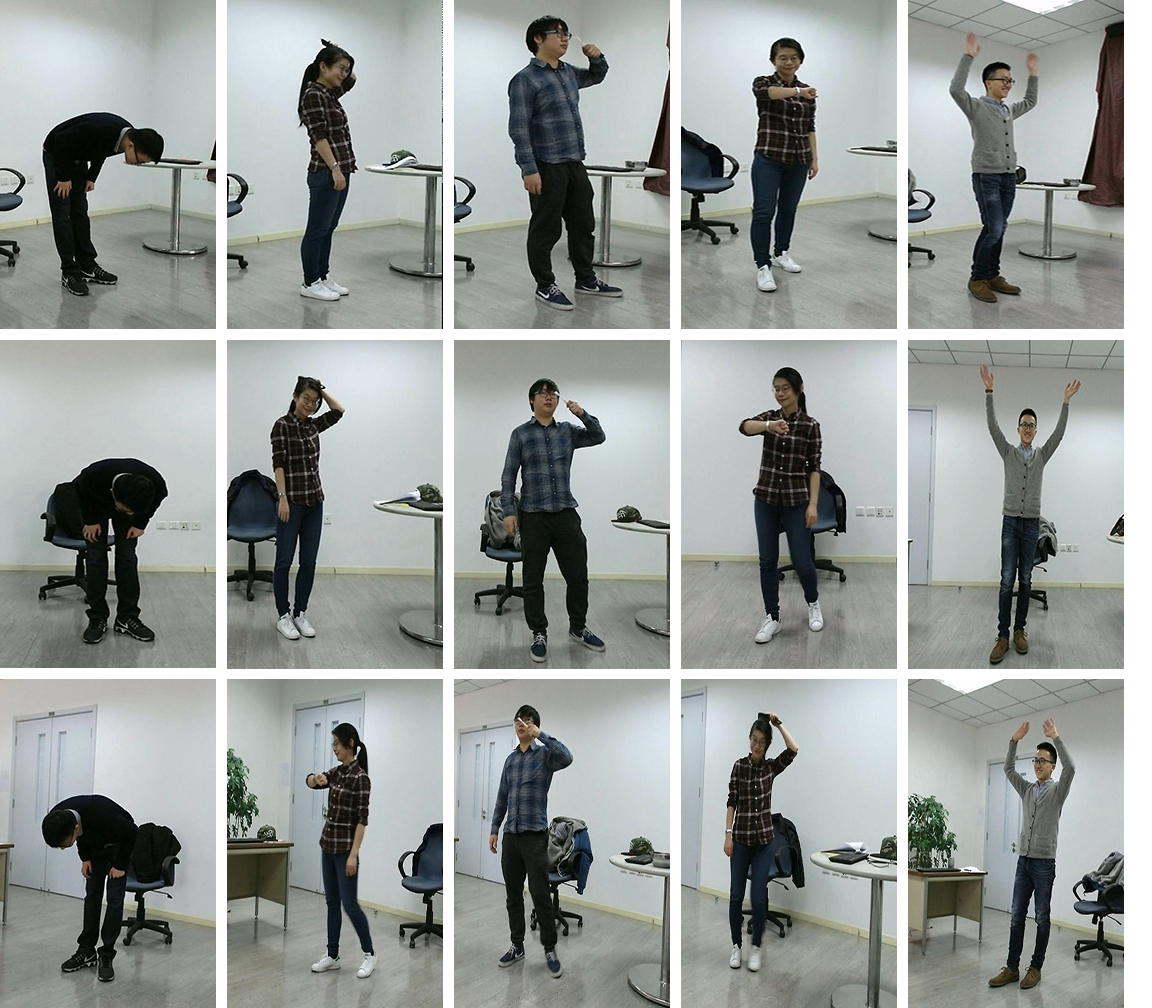
\includegraphics[width=6in,height=4in]{figures/PKUMMD-NEW1}
	\linebreak
	\captionof{figure}{PKU-MMD video sample frames from three different angles.}
	\label{fig1:PKUMMD}
\end{figure}
\section{Data Preprocessing} 
The data preprocessing consist of two steps. In the first step, large videos containing multiple actions are segmented into smaller videos which contain only a single action. Then an object detector is used to detect humans and other objects in video frames. The object detector also gives the bounding box information and based on that information video frames are cropped to remove the background objects, which are not required for the study.
\subsection{Data Segmentation}

The dataset has 1000+ long action sequences, each of which lasts about 3$\sim$4 minutes and has about 20 action instances. For each long action sequence, the data label file is provided that contains the label information for each action in video and the starting and ending frame of an action. Based on the label file information, each video is segmented. After segmenting each view, the dataset has 3,000 minutes video with 20,000+ temporally localized actions. 
\subsection{Video Frame Cropping}

The PKU-MMD dataset is collected through Kinect V2 sensor with a resolution of $1920\times1080$ pixels. While the action setup area is 180 \si{cm} as length and 120 \si{cm} as width. To crop the images, we have to first detect the person in the frame and based on that we have to crop the frames. For the person detection, we used YOLO (You Only Live Once)~\cite{DBLP:journals/corr/RedmonF16} the state-of-the-art, real-time object detection system that can detect over 9000 objects. 

The YOLO does not only detect objects in the video frame, but also labels them as shown in Figure~\ref{fig1:PKUMMD-Example}. It outputs the bounding box positions for each frame. So, in our method, we first used YOLO to detect the person in videos and get the bounding box values for the detected person in each frame. Then, single maximum bounding box value is chosen from all video frames and based on the maximum bounding box size for a person of all videos.
\begin{figure}[!ht]
	\centering
	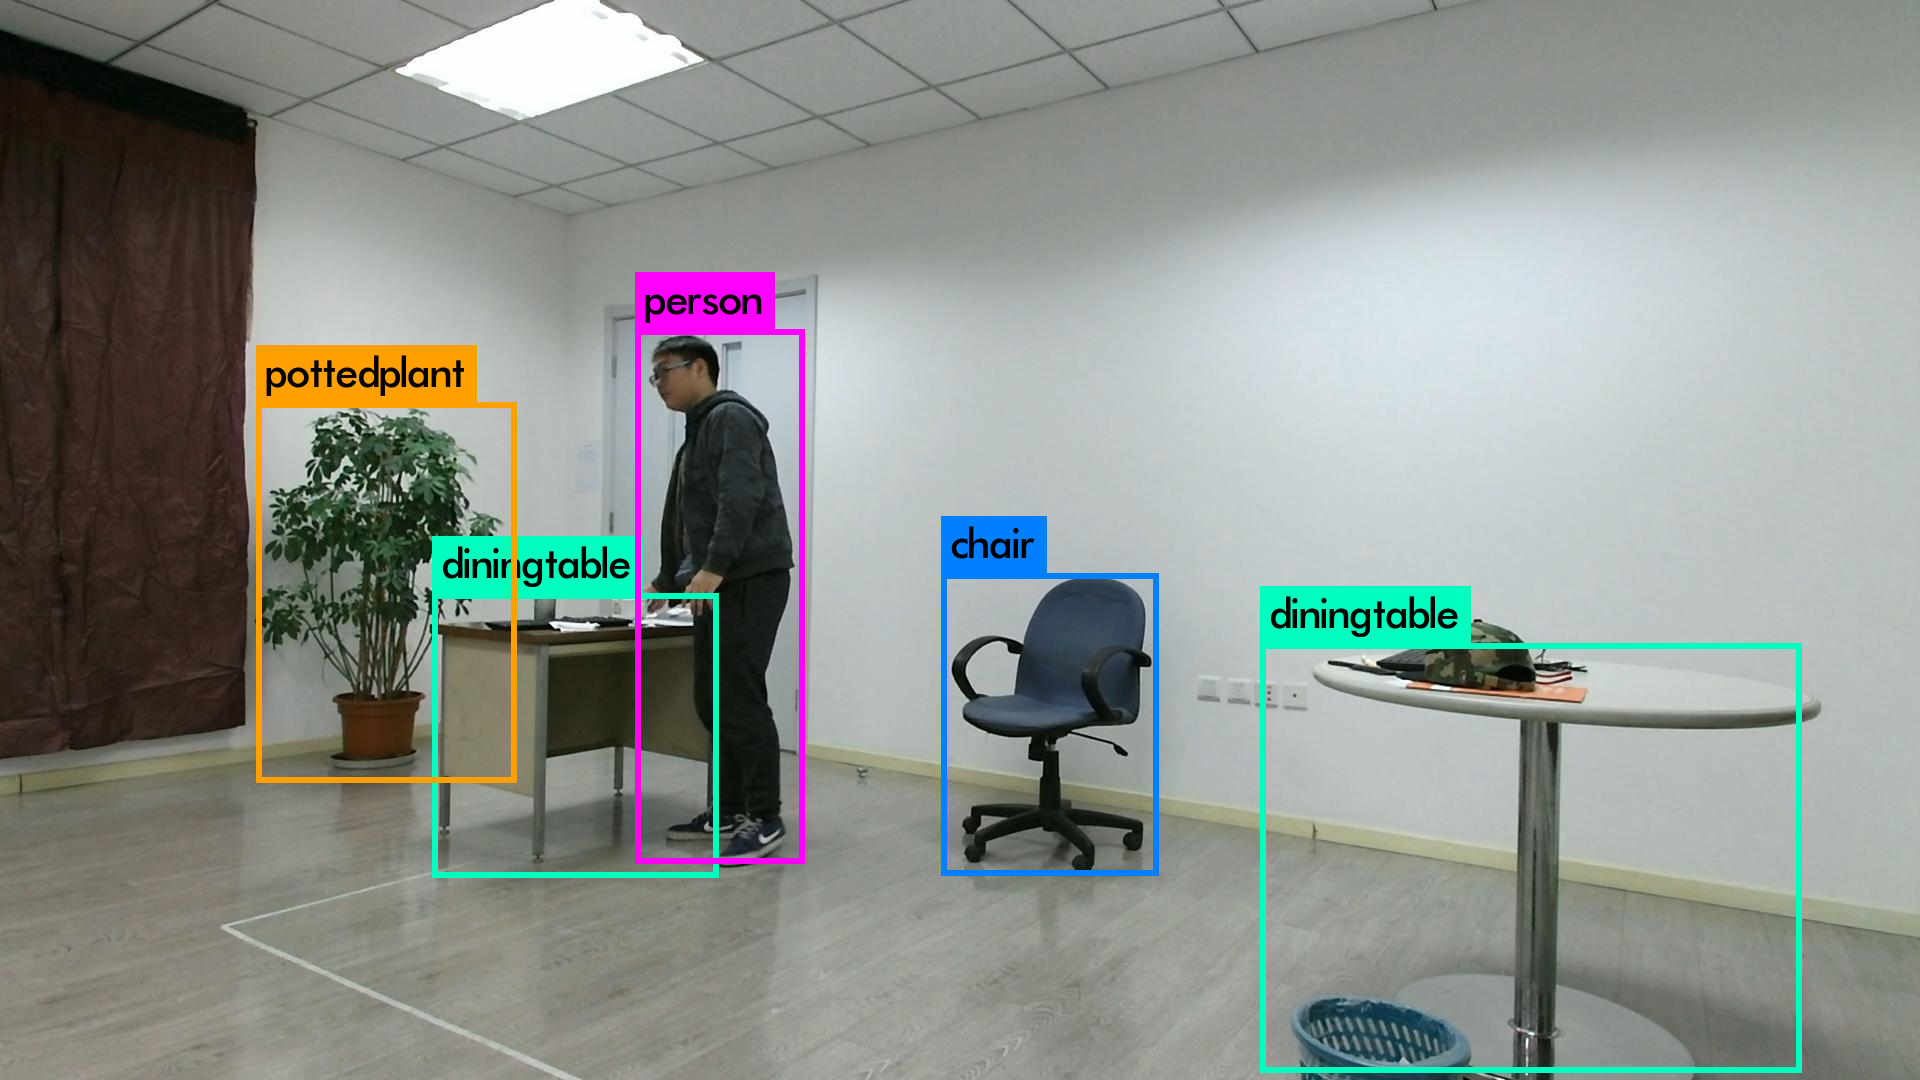
\includegraphics[width=6in,height=4in]{figures/predictions}
	\linebreak
	\captionof{figure}{Detection on PKU-MMD data frame.}
	\label{fig1:PKUMMD-Example}
\end{figure}

\section{Fisher Vector Encoding}
To evaluate the performance of IDT, we used a standard FV approach. A codebook for each descriptor is constructed (trajectory, HOG, HOF, MBH) and a codebook is constructed for the combination of all descriptors. The different number of centers were used which varies from 32 to 256. We fixed it to 64 in our experiments because the performance is very stable compared to other number of centers. 
Note, the FV encoded descriptor dimension for each video is  $1 \times 54528$. To avoid the curse of dimensionality and reduce the computational burden, feature dimensions are further reduced to 400 using PCA. SVM and LibSVM with Linear Kernel are employed for classification.

\section{Experimental Setting}
The IDT code was compiled using the same setting as described in~\cite{HengWang:2011:ARD:2191740.2192078}. We complied this code on 16GB Linux (Ubuntu 16.04) machine with i7-7700k (4.2 GHz). In order to compile the IDT code, Opencv 2.4.11 and ffmpeg-0.11.1 were installed on the machine. The rest of the experiments were performed using MATLAB R2017a. 
%The IDT code is compiled on 16GB Linux machine with i7-7700k (4.2 GHz). In order to compile the IDT code, Opencv 2.4.11 and ffmpeg-0.11.1 were installed on the machine. The rest of the experiments were performed using MATLAB R2017a on 32GB Windows machine with i7-7700k @ 4.2 GHz with 4 cores.









